
\subsection{Environment Set-Up}

\subsubsection{Existing Environments}

The first step towards implementation is to set up a comfortable and adjustable
environment. There are several environments one can use to build Solidity
applications, most popular of which are Truffle(ref), Remix(ref) and
Embark(ref). However, none of the aforementioned applications delivered the
experience we needed in the scope of our project, due to the lack of speed and
customization options. That led us to the creation of a custom environment for
importing, compiling, deploying and testing smart contracts.

We used Python(ref) to build our environment, since it is a powerful and
convenient programming language, and all dependencies we needed had available
Python implementations. We developed our environment in Linux(ref).

\subsubsection{Dependencies}

The components we used as building blocks are Web3(ref) which is a powerful
library for interacting with Ethereum, the Solidity v0.6.6 compiler(ref), and
EthereumTester which is a set of tools for testing Ethereum-based applications.
For the purpose of our project, a private blockchain running an Ethereum
Virtual Machine (EVM) was deployed.  This is a common practice for Ethereum
development since it greatly facilitates testing procedures. Our environment
supports multiple EVMs, namely Geth(ref), Ganache(ref) and Py-EVM(ref).

\subsubsection{Ethereum Virtual Machines}

All aforementioned EVMs deliver implementations that comply with the
specifications described at the Ethereum yellow paper(ref). However, different
implementations provide unique choices to the developer, each of which helped
us to progress effortlessly during different stages of our work.

\paragraph {Py-EVM:} Py-EVM is an evolving EVM which is created mainly for
testing. The ease of access and use, the configuration freedom of its
underlying test chain and its effectiveness for small size of data helped our
first steps. However, as the input data size started to grow, the effectiveness
of the tool rapidly fell(ref).

\paragraph {Ganache:} Ganache is a popular EVM developed by the Truffle team.
Its speed and configuration freedom are its main advantages. However, its
extreme memory requirement made it impossible to use when the sizes of the
input became analogous to the Bitcoin blockchain size.

\paragraph {Geth:} Geth is another popular EVM which is created by the Ethereum
team. It supports heavy customization while its memory usage is very limited
compared to Ganache, even for extensive inputs. It has, however, higher
execution times than Ganache for our purposes because Geth doesn't natively
support auto-mining. That is the capability to mine new blocks only when new
transactions are available. In order to avoid intense use of the CPU, we
injected a function in Geth's \texttt{miner} object be only invoked when a new
transaction is available.  This, together with the fact that mining is
probabilistic, put an extra overhead at the execution time.

\paragraph {Configuration:} We observed that selecting and using an EVM for
testing purposes is not trivial. The set of configurations we used for each EVM
can be found in our public repository(ref). We hope this will facilitate future
work.

\todo{figure of Py-EVM vs Ganache vs Geth}

\subsubsection{Gas Profiling}

Another useful utility we used is solidity-gas-profiler(ref), a profiling
utility by Yushih. This experimental software displays the gas usage in a smart
contract for each line of code. It gave us great insights regarding the gas
usage across contract’s functions, and consequently helped us target the
functionalities that needed to be refined.

\todo{figure of gas profiling}

\subsection{Model}

As mentioned above, we used a previous verifier implementation(ref) as a basis
for our implementation. Since we adopted common primitives, we used some of the
tools Giorgos et al.\ used for functionalities such as constructing blockchains
and proofs. For the purposes of our project, we needed to enhance the
functionality of the existing tools in some cases. We are thankful to the
writers for sharing their implementation. This greatly facilitated our work.

In this subsection, we describe the model that our work shares this the
previous implementation. This includes the following::

\begin{enumerate}
    \item
        Construct a blockchain
    \item
        Construct a proof for an event in the blockchain
    \item
        Verify the proof
\end{enumerate}


\subsubsection{Blockchain}

The tool that creates the blockchain was created by Andrew Miller, one of the
writers of Non-Interactive Proofs of Proof of Work(ref) paper.  The tool is
using the Bitcoin library(ref) to construct a blockchain similar to Bitcoin’s.
The interlink pointers are organized into a Merkle(ref) tree and the index is
determined by their level. For details regarding the level calculation, see
section(ref). The Merkle root of the interlink tree is a 32-bit value, and is
included in the block header as an additional value. The new size of the block
header is 112 bytes. In order to ensure security, it is important for the
interlink root to be included in the block header, as it is part of the proof.
Otherwise, attackers could attack the proofs by reordering or including stray
blocks. Miners can easily verify that the Merkle root is correct.

\todo{figure of blockchain}

\subsubsection{Superblock Levels}

We assume that the difficulty target of mined blocks is constant. As discussed
in section(ref), this is not the actual setting of the Bitcoin blockchain. The
definition of superblocks is changed to a simpler definition and the level is
determined by the number of leading zeros of the block header hash. Although
this change does not take into account the difficulty target, the scoring of
proofs does not generate security holes in the protocol.

\myworries{do we need to justify this?}

\subsubsection{Proof}

The tool that creates proofs was also created by Andrew Miller. The
prover receives the following inputs:

\begin{itemize}
    \item
        A blockchain with interlinks
    \item
        The security parameter $k$
    \item
        The security parameter $m$
\end{itemize}

Security parameters $k$, $m$ are part of the NIPoPoW model and are
explained in section(ref).

The prover’s output is a Proof of Proof of Work that satisfies the above
security parameters. The prover needed to be enhanced in order to create
special test cases (section(ref)) and enable our optimized architecture
(section(ref)).

\todo{figure of proof}

\subsubsection{Verifier}

The goal of the verifier is to securely determine if an event has occurred in
the honest blockchain. For this, the concept of NIPoPoWs is used. A proof is
submitted in combination with a predicate. The proof is considered valid if it
is constructively correct(ref) and the predicate is true for the chain
described by the proof. The predicate represents the existence of an event
in the source blockchain, such as the occurrence of a transaction. In our case,
the predicate indicates the existence of a block in the proof.

\myworries{How much more demanding is to prove an actual transaction?}

The verifier functions in two main phases: (a) \textbf{submit phase} and (b)
\textbf{contest phase}. Each phase has different input and functionality, and
is performed by different entities.

\paragraph{Submit phase:} In \textbf{submit phase}, an entity submits a proof
and an event. We assume that at least one honest full node is aware of the
submission. This is also a part of the model of NIPoPoWs, and is a logical
assumption as explained in the paper. In order to claim the occurrence of an
event, one must provide a proof and a predicate regarding the underlying event.
If $r$ rounds pass, the value of the predicate becomes immutable. The passing
of rounds is indicated by the mining of new blocks atop of the block containing
the submitted proof. The value of the predicate can change if a different entity
successfully contests the submitted proof at some round $r_{c} < r$.

\paragraph{Contesting phase:} In \textbf{contesting phase}, a new proof is
submitted. If this proof is better, then the predicate is evaluated against the
new proof. The contesting proof is considered better only if it is structurally
correct and it represents a chain that encapsulates more Proof of Work than the
originally submitted proof, as described in the NIPoPoWs paper.  In order to
contest, one must provide the new proof and the predicate that is claimed to be
true by the originally submitted proof.\\

The expected functionality of a NIPoPoW verifier is the following:
\begin{itemize}

    \item
        If an \textit{honest} party submits a proof and no contest occurs, then
        the $predicate$ becomes $true$.

    \item
        If an \textit{honest} party submits a proof and it is contested by an
        \textit{adversary}, then the contest should be unsuccessful and the
        $predicate$ should remain $true$.

    \item
        If an \textit{adversary} submits a proof, then an \textit{honest} party
        should make a contest. The contest should invalidate the original
        submission and the $predicate$ should become $false$.

    \item
        The scenario in which an \textit{adversary} submits a proof an
        \textit{honest} does not contest should not take place due to the
        assumption that at least one honest party observes the traffic of the
        contract.

\end{itemize}

\subsubsection{Notation}

In this section we will use the notation displayed in
table~\ref{table:notation}.

\begin{table}[H]
\begin{tabular}{ll}
\hline
\multicolumn{1}{|c|}{Symbol} & \multicolumn{1}{c|}{Description}                       \\ \hline
$E_{submit}$                   & The entity submitting a proof at submit-phase          \\
$E_{cont}$                     & The entity initiating a proof contest at contest-phase \\
$\pi_{orig}$                 & The proof submitted by S                               \\
$\pi_{exist}$                & The copy of $\pi_{orig}$ submitted by C                \\
$\pi_{cont}$                 & The contesting proof submitted by C                    \\
$\pi${[}i{]}                 & The $i$-th superblock of proof $\pi$                  \\
$\pi${[}i:j{]} & The aggregation of superblocks $\pi[i]$, $\pi[i+1]$, ..., $\pi[j-1]$              \\
$\pi${[}i:{]}  & The aggregation of superblocks from $\pi[i]$ until the last block of $\pi$        \\
$\pi${[}:j{]}  & The aggregation of superblocks from the first block of $\pi$ until the $\pi[j-1]$ \\
$\pi\{i, j\}$                & The set of superblocks consisting of $\pi[i,j]$
\end{tabular}
\caption{Notation}
\label{table:notation}
\end{table}


\subsection{Previous Implementation}
\todo{Should it be Previous Work?}

In this subsection we present previous work. We prepare the reader by focusing
at specific aspects in which our solution differs. We will later show these
differences and we will analyse on how they impact the results of our
application.
\chapter{Implementation}

\section{Analysis of Previous Work}
In the process of building our Bitcoin Client, a suit of thorough unit tests
were written to assert the correction of our results which we also used at the
previous work. We discovered some erroneous functionalities that we appose in
subsection \ref{sssc:Security Analysis}
\todo{tests should be more visible}

\subsubsection{Overview} As mentioned in the NIPoPoWs(ref Algorithm 7) paper,
in order to construct a verifier, a Directed Acyclic Graph (DAG) needs to be
maintained in memory. This structure is stored in the form of a hashmap(ref),
and is used to host blocks of all different proofs. This process aims to
prevent adversarial proofs which are structurally valid but blocks are
intentionally skipped. Such a scenario is displayed in
figure~\ref{figure:DAG_usage}. The DAG is then used to construct ancestors
structure by performing a simple graph search. By iterating ancestors, we can
securely determine the value of the predicate.

% \begin{figure}[h!]
    \centering
    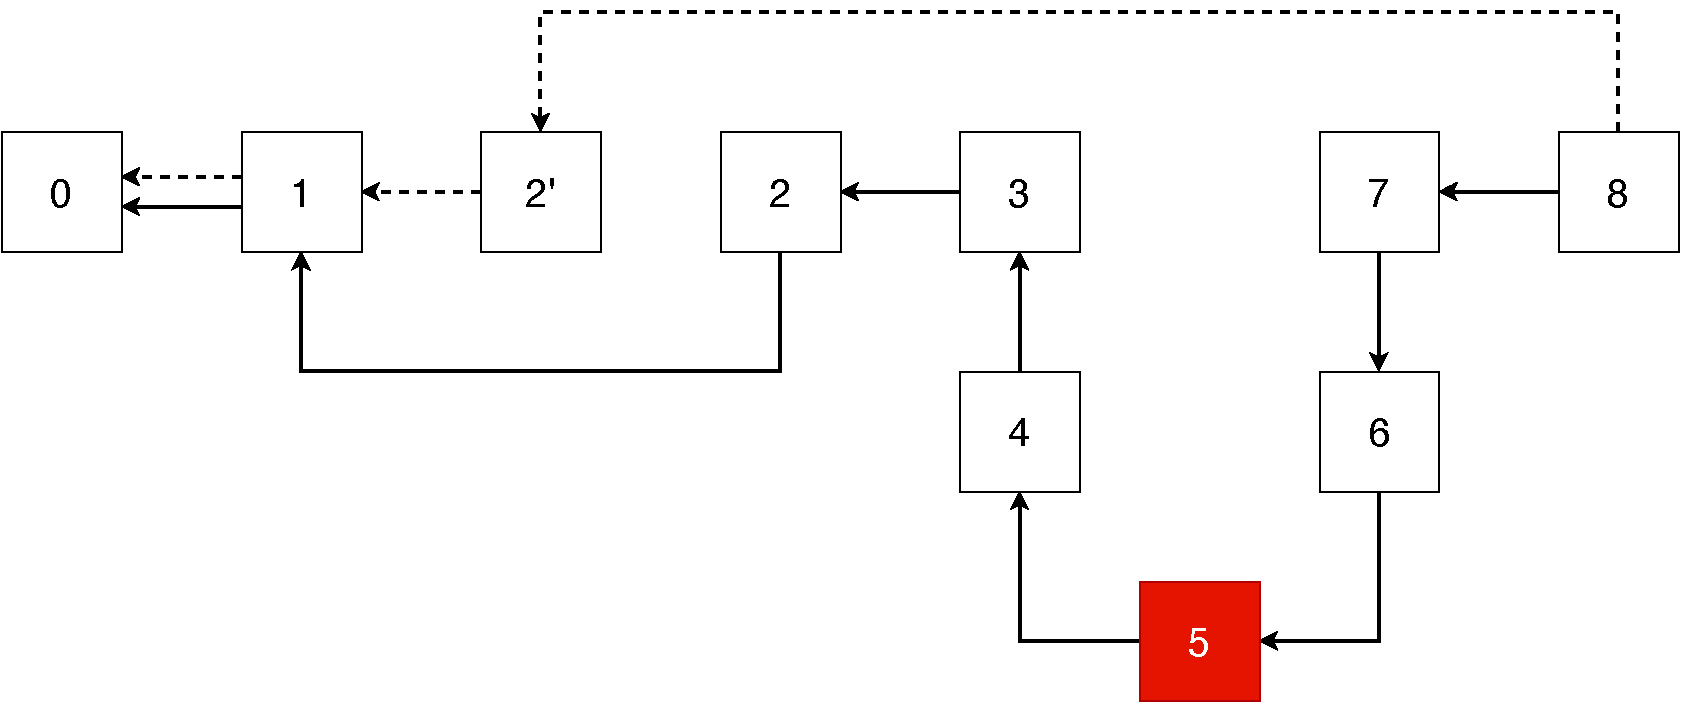
\includegraphics[width=8cm]{./images/DAG_usage.pdf}
    \caption{Combination of multiple proofs in a DAG. The red block is the
        block of interest. Honest proof consists of blocks connected by solid
        lines and adversarial proof by dashed lines. The adversary
        intentionally uses a different set of blocks.}
    \label{figure:DAG_usage}
\end{figure}


This logic is intuitive and efficient to implement in most traditional
programming languages (C++, JAVA, Python, JavaScript, etc). However, such an
algorithm cannot be efficiently implemented in Solidity as is. This is not due
to the lack of features, such as the existence of hashmaps, but because
Solidity treats storage differently than most programming languages. As
mentioned above(ref) in smart contracts the caller needs to pay in gas for the
execution of operations such as accessing and storing data. Reading from and
writing to persistent memory are very expensive operations in Solidity, as
stated in the Ethereum yellow paper(ref). A summary of gas costs for storage
and memory access if is displayed in Table~\ref{table:ethereum_gas_list}. This
fact was observed by Giorgos et al.\ and was recognized as the bottleneck of
the application.

\begin{table}[]
\centering
\begin{tabular}{@{}llr@{}}
\toprule
\multicolumn{1}{c}{Operation} & \multicolumn{1}{c}{Cost} & \multicolumn{1}{c}{Desc} \\
\midrule
$G_{create}$ & 32000 & Paid for a CREATE operation.\\
$G_{sload}$ & 200 & Paid for a SLOAD operation.\\
$G_{sset}$ & 20000 & Paid for an SSTORE operation.\\
$G_{memory}$ & 3 & Paid words expanding memory.\\
$G_{txdatazero}$ & 4 & Paid for zero byte of data for a transaction.\\
$G_{txdatanonzero}$ & 68 & Paid for non-zero byte of data for a transaction.\\
\end{tabular}
\caption{Ethereum gas list}
\label{table:ethereum_gas_list}
\end{table}


\subsubsection{Phases}

We describe each phase of the previous implementation in
Algorithms~\ref{algo:submit_old} and~\ref{algo:contest_old}. We highlight
structures that access persistent memory. Note that deleting from persistent
memory is also considered a storage operation

\begin{algorithm}[H]
    \caption{Submit Event Proof}
    \label{algo:submit_old}
    \KwIn{$proof$, $predicate$}
    \KwData{
        \texttt{array} $proof_{s}$,
        \texttt{hashmap} $DAG_{s}$,
        \texttt{bool} $predicate_{s}$
    }
    require $predicate_{s}$ $=$ $\emptyset$ \\
    require $validInterlink(proof$) \\
    $DAG_{s}$ $\leftarrow$ $DAG_{s}$ $\cup$ $proof$\\
    $proof_{s}$ $\leftarrow$ $proof$\\
    $ancestors_{s}$ $\leftarrow$ $findAncestors(DAG_{s}$)\\
    $predicate_{s}$ $\leftarrow$ $evaluatePredicate(ancestors_{s}$,
    $predicate$)\\
    delete $ancestors_{s}$\\
\end{algorithm}

\begin{algorithm}
    \caption{Submit Contesting Proof}
    \label{algo:contest_old}
    \KwIn{$proof'$, $predicate$}
    \KwData{
        \texttt{array} $proof_{s}$,
        \texttt{hashmap} $DAG_{s}$,
        \texttt{bool} $predicate_{s}$
    }
    require $predicate_{s}$ = $predicate$\\
    $lca$ $\leftarrow$ findLca($proof_{s}$, $proof'$)\\
    require $score(proof’[lca:])$ $>$ $score(proof_{s}[lca:])$ \\
    $DAG_{s}$ $\leftarrow$ $DAG_{s}$ $\cup$ $proof'$\\
    $ancestors_{s}$ $\leftarrow$ $findAncestors(DAG_{s})$\\
    $predicate_{s}$ $\leftarrow$ $evaluatePredicate(ancestors_{s},
    predicate)$\\
    delete $ancestors_{s}$\\
\end{algorithm}


\subsection{Gas analysis}

Here, we layout experiments that show the gas usage of the previous
implementation. In these experiments, we used a small proofs\footnote{For sizes
of proofs for realistic blockchain sizes, refer to Section(ref)}. These sizes
are unrealistic for a real blockchain, but are helpful to demonstrate the gas
of the functions of the contract for each phase. The gas expend for submit and
contest for proof of 20 blocks is shown in Table~\ref{table:old_gas_usage}. We
observe that even for small proofs, the gas cost is high - 4 million gas units,
given that the block gas limit of Ethereum is currently at 9.908.813(ref) gas
units. This is mainly due to the extensive storage usage.

\todo{maybe show numbers for the minimum proof that
exceeds block gas limit.}

\begin{table}[H]
    \centering
    \begin{tabular}{@{}lccll@{}}
        \toprule
        \multicolumn{1}{c}{\textbf{Submit function}} & \textbf{gas usage}    \\ \midrule
        validate Interlink  & \multicolumn{1}{r}{   465,604} \\
        \\
        \\
        store proof         & \multicolumn{1}{r}{ 1,044,705} \\
        store DAG           & \multicolumn{1}{r}{ 3,168,612} \\
        store ancestors     & \multicolumn{1}{r}{ 4,995,289} \\
        evaluate predicate  & \multicolumn{1}{r}{   306,433} \\
        delete ancestors    & \multicolumn{1}{r}{    45,137} \\
        \midrule
        Sum                 & \multicolumn{1}{r}{10,025,780} \\
        \bottomrule
    \end{tabular}
    \quad
    \begin{tabular}{@{}lccll@{}}
        \toprule
        \multicolumn{1}{c}{\textbf{Contest function}} & \textbf{gas usage} \\ \midrule
        validate Interlink  & \multicolumn{1}{r}{   485,751} \\
        find LCA            & \multicolumn{1}{r}{ 1,255,523} \\
        compare proofs      & \multicolumn{1}{r}{   447,130} \\
        store proof         & \multicolumn{1}{r}{   304,845} \\
        update DAG          & \multicolumn{1}{r}{ 1,836,578} \\
        store ancestors     & \multicolumn{1}{r}{ 5,584,173} \\
        evaluate predicate  & \multicolumn{1}{r}{   390,307} \\
        delete ancestors    & \multicolumn{1}{r}{    57,023} \\
        \midrule
        Sum                 & \multicolumn{1}{r}{10,361,330} \\
        \bottomrule
    \end{tabular}
    \caption{Execution for proof of 75 blocks}
    \label{table:old_gas_usage}
\end{table}


\subsection{Security Analysis}

\subsubsection{Pre-mining} We observed that the smart contract is vulnerable to
pre-mining(ref). By definition, a valid NIPoPoW is structurally correct if two
properties are satisfied:

\begin{enumerate}[(a)]

\item The interlink structure of all blocks is correct. This is to prevent
    adversaries from injecting blocks that do not exist in the original
    blockchain.

\item The first block of proof is $genesis$. This is to prevent adversaries
    from create coins before blockchain are advertised at the public network.

\end{enumerate}

The second property is not verified in the previous work, exposing the verifier
to pre-mining attacks. We can easily mitigate this vulnerability by
initializing the smart contract with the $genesis$ block of the blockchain we
will use and add an assertion in submit and contest phase that proofs need to
satisfy property (b). The needed changes are shown in
Algorithms~\ref{algo:avoid_premining_ctor}
and~\ref{algo:avoid_premining_submit}.

\begin{algorithm}[H]

    \caption{\label{alg:avoid-premining}The \textsf{NIPoPoW} client mitigation
    to premining attack}
    \begin{algorithmic}[1]

    \Contract{crosschain}
    \State $\textsf{events} \gets \bot$; $\genesis \gets \bot$
    \State $\textsf{DAG} \gets \bot$; $\textsf{ancestors} \gets \bot$
    \Function{\sf initialize}{$\genesis_{remote}$}
        \State $\genesis$ $\gets \genesis_{remote}$
        \Comment{initialize with the genesis of the underlying chain}
    \EndFunction
    \Function{\sf submit}{$\pis$, $e$}
        \State \textsf{require}($\pis$[0] = $\genesis$)
        \Comment{assert correct genesis}
        \State \textsf{require}($\textsf{events$[e]$} = \bot$)
        \State \textsf{require}($\textsf{valid-interlinks}(\pi)$)
        \State \textsf{events$[e].\pi$} $\gets$ $\pis$
        \State \textsf{DAG} $\gets$ \textsf{DAG} $\cup$ $\pi$
        \State \textsf{ancestors} $\gets$ \textsf{find-ancestors(DAG, $\pi$[-1])}
        \State \textsf{require}(\textsf{evaluate-predicate}(\textsf{ancestors}, e))
        \State \textsf{ancestors} $=$ $\bot$
        \EndFunction
    \Function{\sf contest}{$\pic$, $e$}
        \State \textsf{require}($\pic$[0] = $\genesis$)
        \Comment{assert correct genesis}
        \State \textsf{require}(\textsf{events}$[e]$ $\ne$ $\bot$)
        \State \textsf{require}(\textsf{valid-interlinks}($\pic$))
        \State $lca$ = \textsf{find-lca}($\textsf{events}[e].\pi$, $\pic$)
        \State \textsf{require}($\pic$ $\geq_m$ $\textsf{events}[e].\pi$)
        \State \textsf{DAG} $\gets$ \textsf{DAG} $\cup$ $\pic$
        \State \textsf{ancestors} $\gets$
        \textsf{find-ancestors}($\textsf{DAG}$, $\textsf{events}[e].\pi$[-1])
        \State \textsf{require}($\neg$\textsf{evaluate-predicate}(\textsf{ancestors}, $e$))
        \State \textsf{ancestors} $=$ $\bot$
        \State \textsf{events$[e]$} $\gets$ $\bot$
    \EndFunction
    \EndContract
    \vskip8pt
    \end{algorithmic}
\end{algorithm}



\subsubsection{Score Calculation}

During our tests, we observed that the calculation of proofs score was
incorrect. The score of each level is needed to determine which proof
represents the chain with the most Proof of Work. Between two proofs, we only
need to calculate the score starting from their $lca$ until the tip of each
proof. Different levels are needed because the $lca$ between two proofs is only
known when the contesting proof is submitted. The security parameter $m$ needs
to be satisfied for every sub-proof $\pi[:lca]$. We ensure that this is $true$
by creating proofs of multiple levels, so that security parameter $m$ applies,
disregarding $lca$'s position.

\todo{Figure for the need of multiple levels}

Each block has a level, calculated as describe in Section(ref)
\[ level = getLevel(block) \]
Consequently, each level of the proof consists of a number of blocks
$n_{level}$. This number is the sum of blocks of level $\geq$ $level$, i.e.\
block of level $l$ are also blocks of levels $l-1$, $l-2$, etc. The
score of each level is computed as:

\[score_{level} = 2^{level} \times n_{level}\]

After running out tests for the previous implementation, we observed that
function $getLevel(block)$ of the contract was returning $block.level-1$
instead of $block.level$ resulting to incorrect score computation. This can
prevent an honest party from successfully contesting an adversarial proof,
making the contract insecure. The function was refined to return the correct
value.

\section{Storage Elimination}
\todo{Should this be a new section?}

As mentioned above, the bottleneck we had to eliminate was the extensive usage
of storage. We created a new architecture that allow us to discard all
expensive store operations and utilize memory instead. This led to massive
decrease of gas consumption. In this section, we present the difference in gas
usage between storage and memory utilization, and how a NIPoPoW verifier can be
implemented in Solidity without persisting proofs.

\subsection{Storage vs Memory}

We will first demonstrate the difference in gas usage between storage and
memory for a smart contract in Solidity. Suppose we have the following simple
contract:

\lstinputlisting[style=customc, captionpos=b, label={listing:storage_memory},
caption={Solidity test for storage and memory}]{code/StorageVsMemory.sol}
\todo{Highlight code}

Function \texttt{withStorage()} populates an array saved in storage and
function \texttt{withMemory()} populates an array saved in memory. We
initialize the sizes of the arrays by passing the variable \texttt{size} to the
contract constructor. We run this piece of code for \texttt{size} from 1 to
100. The results are displayed at Figure~\ref{figure:memory_vs_storage}. For
\texttt{size} = 100, the gas expended is 53,574 gas units using memory and
2,569,848 using storage which is almost 50 times more expensive. This code was
compiled with Solidity version 0.6.6 with optimizations enabled\footnote{This
version of Solidity compiler, which was the latest at the time this paper was
published, did not optimize-out any of the variables.}. The EVM we used  was
Ganache at the latest Constantinople(ref) fork. It is obvious that if there is
the option to use memory instead of storage in the design of smart contracts,
the choice of memory greatly benefits the users.

\begin{figure}
\centering
\begin{tikzpicture}
    \begin{axis}[
        y tick label style={/pgf/number format/.cd,%
          set thousands separator={,},
          fixed},
        legend pos=north west,
        scaled y ticks = false,
        grid=major,
        xlabel={Array size},
        ylabel={Gas consumption}]
    \addplot table [mark=none, col sep=comma] {data/storage.csv};
    \addplot table [mark=none, col sep=comma] {data/memory.csv};
    \legend{$storage$,$memory$};
\end{axis}
\end{tikzpicture}
\caption{Gas consumption for memory and storage}
\label{figure:memory_vs_storage}
\end{figure}


\subsection{Making use of calldata}

In previous work we needed to store submitted proofs in order to proceed to
contest. In this subsection we show an approach to securely verify proofs
without utilizing the persistent storage of the smart contract.

The rationale is to demand from the caller to provide two proofs to the
contract during contest phase: (a) $\pi_{exist}$, which is a copy of the
originally submitted proof $\pi_{orig}$, and (b) $\pi_{cont}$, which is the
contesting proof. Proof $\pi_{orig}$ can be retrieved by observing contract's
\textit{calldata}. We prevent an adversary from malforming $\pi_{exist}$ by
storing the hash of $\pi_{orig}$ to contract's state during submit phase and
then verifying that $\pi_{exist}$ has the same hash. The operation of hashing
the proof and storing the digest is cheap\footnote{By setting $k=6$, $m$ = 13,
a proof for the entire Bitcoin blockchain consists of less than 300
superblocks. The hashing of such a proof costs approximately 300,000 gas
units.} as shown in figure~\ref{figure:hash_proof_gas}. We calculate the digest
of the proof by:

\[\texttt{digest = sha256(abi.encodePacked(proof))}\] The size of the digest of
a hash is 32 bytes. To persist such a small value in contract's memory only
adds a constant, negligible cost overhead to our implementation.

\begin{figure}
\centering
\begin{tikzpicture}
    \begin{axis}[
        y tick label style={/pgf/number format/.cd,%
          set thousands separator={,},
          fixed},
        legend pos=north west,
        scaled y ticks = false,
        grid=major,
        xlabel={Proof size},
        ylabel={Gas consumption}]
    \addplot table [col sep=comma] {data/hash_proof_gas.csv};
    \legend{sha256 gas cost};
\end{axis}
\end{tikzpicture}
\caption{Gas consumption for hashing proofs and storing digest}
\label{figure:hash_proof_gas}
\end{figure}



\subsection{Removing DAG and ancestors}

As shown in table~\ref{table:old_gas_usage}, the most demanding operation is
the creation and population of DAG and ancestors. In this subsection we show
how these two structures can be discarded from the verifier.

\subsubsection{Using subset} Our first realization was that instead of storing the
DAG of $\pi_{exist}$, $\pi_{cont}$, we can require

\[ \pi_{exist}\{:lca_{e}\} \subseteq \pi_{cont}\{:lca_{c}\} \]
where $lca_{e}$ and $lca_{c}$ are the indices of the $lca$ block in
$\pi_{exist}$, and $\pi_{cont}$, respectively. This way we avoid
the demanding need of composing auxiliary structures DAG and ancestors
on-chain. The implementation of \texttt{subset} is displayed in
listing~\ref{listing:subset}. The complexity of the function is
\[ \mathcal{O}(\mid\pi_{exist}[:lca_{e}]\mid + \mid\pi_{cont}[:lca_{c}]\mid) \]

\lstinputlisting[style=customc, captionpos=b, label={listing:subset},
caption={Implementation of subset}]{code/Subset.sol}

\begin{figure}[ht]
\begin{subfigure}{.5\textwidth}
  \centering
  % include first image
  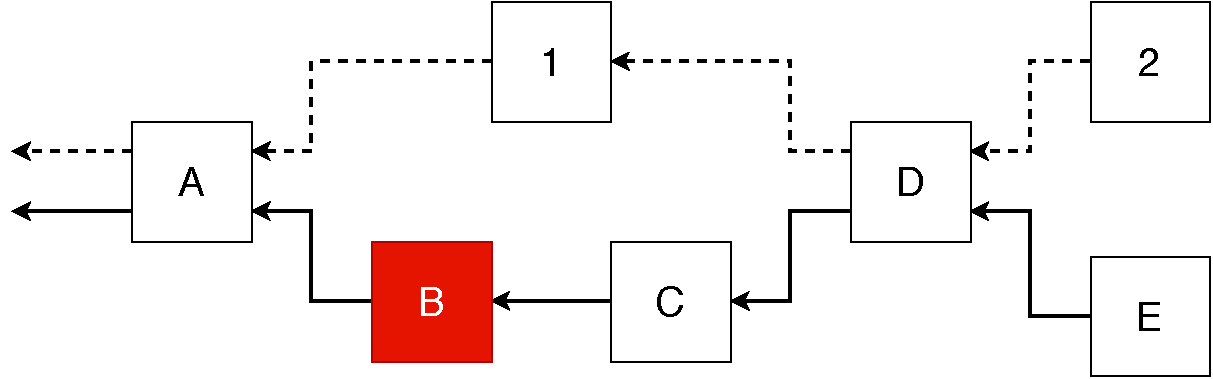
\includegraphics[width=6cm]{../images/Subset_1.pdf}
  \caption{Valid $\pi_{cont}$ before using subset}
  \label{figure:DAG_usage}
\end{subfigure}
\begin{subfigure}{.5\textwidth}
  \centering
  % include second image
  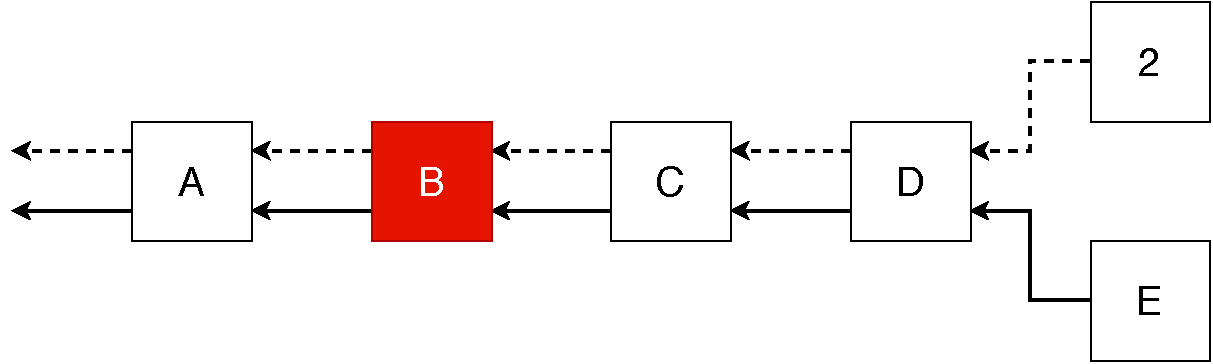
\includegraphics[width=6cm]{../images/Subset_2.pdf}
  \caption{Valid $\pi_{cont}$ after using subset}
  \label{figure:DAG_usage}
\end{subfigure}
\caption{Blocks connected with solid lines indicate $\pi_{exist}$ and blocks
connected with dashed lines indicate $\pi_{cont}$}
\label{fig:fig}
\end{figure}


The gas consumption difference between $subset$ and $DAG + ancestors$ is
displayed at figure~\ref{figure:DAG_vs_subset}. $Subset$ solution is
approximately 2.7 times more efficient.

\begin{figure}
\centering
\begin{tikzpicture}
    \begin{axis}[
        y tick label style={/pgf/number format/.cd,%
          set thousands separator={,},
          fixed},
        legend pos=north west,
        scaled y ticks = false,
        grid=major,
        xlabel={Proof size},
        ylabel={Gas consumption x 1.000}]
    \addplot table [col sep=comma] {data/DAG_ancestors.csv};
    \addplot table [col sep=comma] {data/subset.csv};
    \legend{$DAG+ancestors$,$Subset$};
\end{axis}
\end{tikzpicture}
\caption{Gas consumption for DAG+ancestors and subset}
\label{figure:DAG_vs_subset}
\end{figure}


\subsubsection{Subset complexity and limitations} Requiring $\pi_{exist}$ to be a subset of
$\pi_{cont}$ greatly reduces gas, but the complexity of the $subset$ algorithm
is high since both proofs have to be iterated from genesis to their respective
$lca$ index. Generally, we expect for an adversary to provide a proof of a
chain that is a fork of the honest chain at some point relatively close to the
tip. This is due to the fact that the ability of an adversary to sustain a fork
chain is exponentially weakened as the honest chain progresses.  This means
that the length of $\pi$, $\mid\pi\mid$ is be considerably close to
$\mid\pi[:lca]\mid$, and the complexity of \texttt{subset()} is effectively
$\mathcal{O}(2\mid\pi\mid)$.

In realistic cases, where the $lca$ lies around index 250 of the proof, the gas
cost of \texttt{subset()} is approximately 20,000,000 gas units, which makes it
inapplicable for real blockchains since it exceeds the block gas limit of
the Ethereum blockchain by far.

\subsubsection{Position of block of interest}

By analyzing the benefits and trade-offs of $subset$, we concluded that there
is a more efficient way to treat storage elimination. In general, the concept
of $subset$ facilitated the case in which the block of interest belongs in the
sub-proof $\pi_{exist}[:lca_{e}]$. But in this case, both $\pi_{exist}$ and
$\pi_{cont}$ contain the block of interest at some index, as can be seen in
figure~\ref{figure:after_subset}. Consequently, $\pi_{cont}$ cannot contradict
the existence of the block of interest and the predicate is evaluated $true$
for both proofs. This means that if (a) $\pi_{exist}$ is structurally correct
and (b) the block of interest is in $\pi_{exist}[:lca_{e}]$, then we can safely
conclude that contesting with $\pi_{cont}$ is redundant. Therefore,
$E_{contest}$ can simply send $\pi_{cont}$[lca:] to the verifier. The
truncation of $\pi_{cont}$ to $\pi_{cont}[lca_{c}:]$ can be easily addressed
from $E_{cont}$, since $\pi_{exist}$ is accessible from the contract's
calldata and both proofs can be iterated off-chain.

\newcommand*{\exist}{$\pi_{exist}$}
\newcommand*{\cont}{$\pi_{cont}^{tr}$}

\subsubsection{Disjoint proofs}

We will refer to the truncated contesting proof as $\pi_{cont}^{tr}$ and to
$lca_{e}$ simply as $lca$. For the aforementioned, the following statements are
true:

\begin{enumerate}[(a)]
    \item  $\pi_{exist}[0]$ = $genesis$
    \item  $\pi_{exist}[lca]$ = $\pi_{cont}^{tr}[0]$
\end{enumerate}

The requirement that needs to be satisfied is
\[\pi_{exist}\{lca+1:\} \cap \pi_{cont}^{tr}\{1:\} = \emptyset \]

The implementation of this operation is shown in
listing~\ref{listing:disjoint}.

\lstinputlisting[style=customc, captionpos=b, label={listing:disjoint},
caption={Implementation for disjoint proofs}]{code/Disjoint.sol}

The complexity of \texttt{disjoint()} is
\[ \mathcal{O}(\mid\pi_{exist}[lca_{e}:]\mid \times
\mid\pi_{cont}^{tr}\mid) \]

% \subsection{Fixing vulnerabilities and restricting gas usage}
%
% \begin{itemize}
%
%     \item
%         This is not vulnerable to DOS attacks
%
% \end{itemize}

\pagebreak
